\section{Podstawowe informacje dotyczące przetwarzania obrazów}
\subsection{Podstawowe definicje}
\subsubsection{Piksel}
Piksel jest najmniejszym elementem obrazu cyfrowego. Piksel może określać
\begin{itemize}
\item odcień szarości
\item kolor, wtedy \(f(x, y) = [a(x, y), b(x, y),...]\)\\
  gdzie $a, b,...$ to natężenie poszczególnych barw
\item wskaźnik na element tablicy barw
\end{itemize}
\subsubsection{Obraz cyfrowy}
Obraz cyfrowy jest macierzą pikseli, postaci
\begin{gather*}
  f = f(x, y), x = 0,1,2,...,N-1; y = 0,1,2,...,M-1
\end{gather*}
gdzie
\begin{itemize}
\item \(f(x, y)\) - pojedynelement macierzy, piksel
\item \(M, N\) - szerokość oraz wysokość obrazu
\end{itemize}
\subsubsection{Obraz binarny}
Obraz binarny jest to obraz cyfrowy którego składowe piksele przyjmują wartości
\begin{gather*}
  f(x, y) = z, z \in {0, 1}
\end{gather*}.
\subsection{Podstawowe algorytmy przetwarzania obrazów}
\subsubsection{Operacje morfologiczne}
Operacje morfologiczne na obrazach binarnych wykoszystywane są do filtracji morfologicznej oraz analizy kształtów obiektów na obrazie. Algorytmy morfologiczne są podstawą dla wielu bardziej złożonych algorytmów analizy wizji komputerowej.
\paragraph {Dylatacja obrazu} to rozszerzenie obrazu wykorzystując zadany element strukturalny. Operacja definiowana jest wzorem
\begin{gather*}
  A \oplus B \equiv \bigcup \limits_{b \in B} A_b
\end{gather*}.
Przykładowy wynik operacji dylatacji przedstawiony jest na rysunku~\ref{fig:dilate}.
\begin{figure}
  \centering
  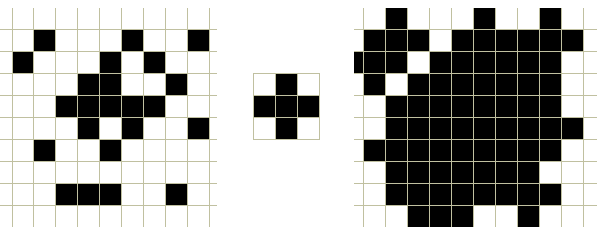
\includegraphics[width=15cm]{img/dilate}
  \caption{Obraz binarny poddany procesowi dylatacji z zadanym elementem strukturalnym}
  \label{fig:dilate}
\end{figure}
\paragraph {Erozja obrazu} to usuwanie zwężanie obrazu z wykorzystaniem zadanego elementu strukturalnego. Operacja definiowana jest wzorem
\begin{gather*}
  A \ominus B \equiv \bigcap \limits_{b \in B} A_{-b}
\end{gather*}.
Przykładowy wynik operacji erozji obrazu przedstawiony został na rysunku~\ref{fig:erode}.
\begin{figure}
  \centering
  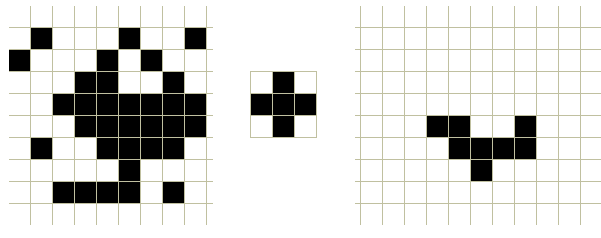
\includegraphics[width=15cm]{img/erode}
  \caption{Obraz binarny poddany procesowi erozji z zadanym elementem strukturalnym}
  \label{fig:erode}
\end{figure}
\paragraph {Zamknięcie i otwarcie obrazu} to złożenie dwóch wyżej wymienionych operacji (dylatacji oraz erozji) w odpowiedni sposób.
\begin{itemize}
\item zamknięcie obrazu definiowane jest w następujący sposób:
  \begin{gather*}
    A \bullet B = (A \oplus B) \ominus B
  \end{gather*}, czyli najpierw wykonywana jest operacja dylatacji obrazu, a następnie przekształcony obraz poddawany jest operacji erozji
\item otwarcie obrazu definiowane jest wzorem:
  \begin{gather*}
    A \circ B = (A \ominus B) \oplus B
  \end{gather*}. W przypadku algorytmu otwarcia obrazu, w pierwszej kolejności wykonywana jest operacja erozji, a następnie opracja dylatacji obrazu.
\end{itemize}
Na rysunku~\ref{fig:open_close} przedstawiony został wynik działania obydwu algorytmów na tym samym obrazie, z tym samym elementem strukturalnym.
\begin{figure}
  \centering
  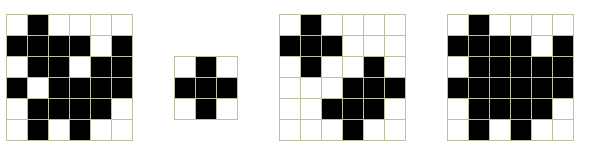
\includegraphics[width=15cm]{img/open-close}
  \caption{Obraz binarny poddany operacji otwarcia oraz zamknięcia obrazu, dla takiego samego elementu strukturalnego}
  \label{fig:open_close}
\end{figure}
\subsubsection{Progowanie}
Progowanie polega na podziale pikseli obrazu na dwie grupy, poprzez wybranie określonej wartości progowej $t$. Każdy piksel jest porównywany z wartością progową, i w zależności od tego, czy wartość piksela jest większa od wartości progowej, czy mniejsza, w tej samej pozycji nowo powstałego obrazu, przypisuje się wartość $1$, lub $0$. Operację można opisać wzorem:
\begin{gather*}
  I_{out}(x, y) = \left\{\begin{matrix}
      1, dla \: I_{in}(x, y) > t\\
      0, dla \: I_{in}(x, y) \leq t
    \end{matrix}\right. x=0,1,2,...,N-1; y=0,1,2,...,M-1
\end{gather*},
gdzie:
\begin{itemize}
  \item $I_{in}$ - obraz wejściowy
  \item $I_{out}$ - obraz wyjściowy
  \item $N$ - szerokość obrazu
  \item $M$ - wysokość obrazu
\end{itemize}
Na rysunku ~\ref{fig:lena_threshold} przedstawiony został wynik operacji progowania na przykładowym obrazie monochromatycznym.
\begin{figure}
  \centering
  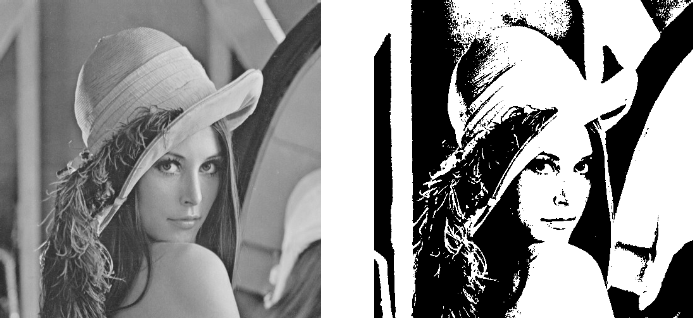
\includegraphics[width=15cm]{img/lena-threshold}
  \caption{Wynik działania operacji progowania z wartością progu $t=128$ dla 8-bitowego obrazu monochromatycznego}
  \label{fig:lena_threshold}
\end{figure}
\paragraph{Progowanie obrazów z większą ilością składowych}\mbox{}\\
Zazwyczaj operacji progowania poddawane są obrazy jednokanałowe. Istnieje jednak możliwość wykonania operacji dla obrazów wielokanałowych (np. dla obrazów RGB). Operacja ta definiowana jest następującym wzorem:
\begin{gather*}
  I_{out}(x, y) = \left\{\begin{matrix}
      1, \; \text{jeżeli} \; \forall c \in C, \; I_{in}(x, y, c) > t(c)\\
      0, \; \text{jeżeli} \; \exists c \in C, \; I_{in}(x, y, c) \leq t(c)
    \end{matrix}\right.\\ x=0,1,2,...,N-1; y=0,1,2,...,M-1; c=0,1,2,...,C
\end{gather*},
gdzie $C$ to liczba kanałów w obrazie.
Algorytm progowania operujący na wielu kanałach może zostać wykorzystany, kiedy znana jest dokładna barwa badanego obiektu.

\subsubsection{Rozmycie obrazu}
Algorytmy rozmycia stosuje się w celu usunięcia z obrazu szumów oraz zbędnych detali. Rozmycie polega na zastosowaniu dla każdego piksela w obrazie funkcji przyjmującej jako argument dany piksel wraz z jego najbliższym sąsiedztwem (tzw. jądro). Powszechnie stosuje się następujące funkcje rozmycia:
\begin{itemize}
  \item mediana,
  \item średnia,
  \item Gauss.
\end{itemize}
Jądro zastosowane w filtrze może mieć dowolne kształty i rozmiary, natomiast w przypadku dużych jąder, algorytm będzie wykonywał się znacznie dłużej, a obraz może zostać rozmyty zbyt bardzo (utracone zostaną istotne informacje zapisane w wejściowym obrazie).
Rysunek~\ref{fig:lena_smooth} przedstawia zaszumiony obraz oraz wynik działania algorytmu rozmycia medianowego.
\begin{figure}
  \centering
  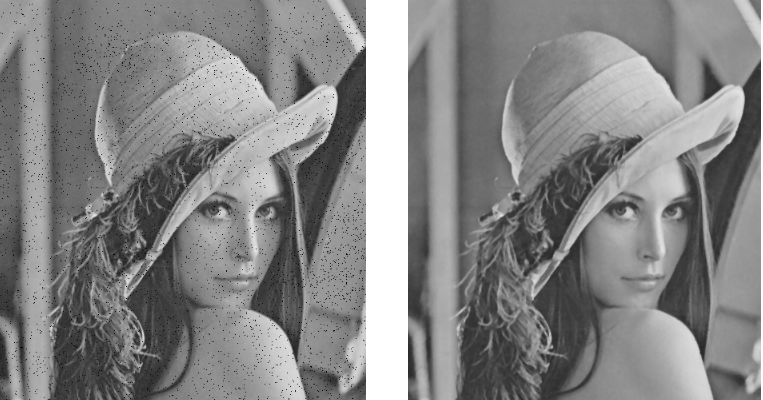
\includegraphics[width=15cm]{img/lena-smooth}
  \caption{Wynik działania filtra rozmycia medianowego z jądrem w kształcie kwadratu 3x3}
  \label{fig:lena_smooth}
\end{figure}
